% =============================================
% =============================================
% Document class: Article
\documentclass[ a4paper, twoside, 11pt]{article}
% Packages: LaTeX (Depth-1)
\usepackage[ vlined, linesnumbered, ruled]{algorithm2e}
\usepackage{ amsfonts, amsmath, amssymb, amsthm}
\usepackage[ titletoc, title]{appendix}
\usepackage{ bbm}
\usepackage{ color}
\usepackage{ dsfont}
\usepackage{ enumitem}
\usepackage{ graphicx}
\usepackage{ fancyhdr, float, fullpage}
\usepackage{ hyperref}
\usepackage{ lastpage, latexsym, lipsum}
\usepackage{ mathrsfs, mathtools, multicol}
\usepackage{ parskip}
\usepackage{ setspace, stmaryrd, subcaption}
\usepackage{ tabularx}
\usepackage{ wasysym}
\usepackage[ dvipsnames, table]{ xcolor}
\usepackage{ xfrac}
% Packages: LaTeX (Depth-2)
\usepackage{ epstopdf}

% =============================================
\topmargin 			= -1.6cm
\headheight 		= .90cm
\headsep 			= .80cm
\textheight 		= 24.0cm
\textwidth 			= 15.5cm
\oddsidemargin		= 0.cm
\evensidemargin 	= 0.cm

% =============================================
% =============================================
% Macros: Language
\newcommand{\define}{\triangleq}
\newcommand{\done}{\hfill $\square$}
%\newcommand{\eqCIRC}{\stackrel{\circ}{=}}
%\newcommand{\eqSTAR}{\stackrel{*}{=}}
\renewcommand{\epsilon}{\varepsilon}
\newcommand{\eg}{\textit{e.g.,\;}}
\newcommand{\egc}{\textit{e.g.:\;}}
\newcommand{\Eg}{\textit{E.g.,\;}}
\newcommand{\Egc}{\textit{E.g.:\;}}
\newcommand{\ie}{\textit{i.e.,\;}}
\newcommand{\iec}{\textit{i.e.:\;}}
\newcommand{\Ie}{\textit{I.e.,\;}}
\newcommand{\Iec}{\textit{I.e.:\;}}
\newcommand{\QED}{\hfill $\blacksquare$}
\renewcommand{\tilde}[1]{\widetilde{#1}}
\newcommand{\tsup}[1]{\ensuremath{^{\text{#1}}}}
\newcommand{\tsub}[1]{\ensuremath{_{\text{#1}}}}
\renewcommand{\vec}[1]{{\boldsymbol{#1}}}

% Macros: Optimization & Probability
\DeclareMathOperator*{\argmax}{arg\,max}
\DeclareMathOperator*{\argmin}{arg\,min}
\newcommand{\Exp}{\mathbb{E}}
\newcommand{\Indicate}[1]{ \IndFun \, \{ \, #1 \, \} }
\renewcommand{\Pr}{\mathbb{P}}
\newcommand{\Normal}{\mathcal{N}}
\newcommand{\std}{\text{std}}
\newcommand{\var}{\text{var}}

% Macros: Sets
\newcommand{\Complex}{\mathbb{C}}
\renewcommand{\emptyset}{\varnothing}
\newcommand{\Nat}{\mathbb{N}}
\renewcommand{\Re}{\mathbb{R}}
\newcommand{\ReNN}{{\Re}_{\geq 0}}
\newcommand{\ReSP}{{\Re}_{> 0}}
\renewcommand{\subset}{\subseteq}
\renewcommand{\supset}{\supseteq}
\newcommand{\Z}{\mathbb{Z}}
\newcommand{\ZNN}{{\Z}_{\geq 0}}

% Macros: Spacing & Other Commands
\newcommand{\fullcut}{\vspace{-\baselineskip}}
\newcommand{\fullskip}{\vspace{\baselineskip}}
\newcommand{\halfcut}{\vspace{-0.5\baselineskip}}
\newcommand{\halfskip}{\vspace{0.5\baselineskip}}
\renewcommand{\figurename}{Figura}
\renewcommand{\tablename}{Tabla}

% =============================================
% Sesion de Clase
\newcommand{\sesion}{05}
% Macros para definiciones, teoremas, etc
\newcounter{sesion}
\setcounter{sesion}{\sesion}
\theoremstyle{definition}
\newtheorem{definition}{Definici\'on}[sesion]
\newtheorem{example}[definition]{Ejemplo}
\newtheorem{exercise}[definition]{Ejercicio}
\newtheorem{note}[definition]{Nota}
\newtheorem{problem}[definition]{Problema}
\newtheorem{theorem}[definition]{Teorema}

% =============================================
% =============================================
\newcommand{\HeaderLine}{}
\newcommand{\FooterLine}{P\'agina \thepage ~de \pageref*{LastPage}}

\pagestyle{fancyplain}
\fancyhf{}

\rhead[]{\fancyplain{}{\HeaderLine}}
\lhead[\fancyplain{}{\HeaderLine}]{}
\lfoot[\fancyplain{}{\FooterLine}]{}
\rfoot[]{\fancyplain{}{\FooterLine}}

\renewcommand{\headrulewidth}{0.4pt}
\renewcommand{\footrulewidth}{0.4pt}
\renewcommand{\thefootnote}{\fnsymbol{footnote}}

% =============================================
% =============================================
\begin{document}
\allowdisplaybreaks

\begin{center}
\Large Control Autom\'atico: Lecci\'on \sesion \\[1ex]
\small \textbf{A\~no:} 2016-2017 \qquad \textbf{T\'ermino:} II \qquad
\textbf{Instructor:} Luis I. Reyes Castro \qquad \textbf{Paralelo:} 02
\end{center}
\halfskip

\fbox{

\begin{minipage}[b][\height][t]{\textwidth}
\vspace{0.2 cm}

\begin{center}
\textbf{COMPROMISO DE HONOR}
\end{center}
\vspace{0.4 cm}

\scriptsize
{
Yo, \rule{60mm}{.1pt} al firmar este compromiso, reconozco que la presente lecci\'on est\'a dise\~nada para ser resuelta de manera individual, que puedo usar un l\'apiz o pluma y una calculadora cient\'ifica, \linebreak que solo puedo comunicarme con la persona responsable de la recepci\'on de la lecci\'on, y que cualquier instrumento de comunicaci\'on que hubiere tra\'ido debo apagarlo. Tambi\'en estoy conciente que no debo consultar libros, notas, \linebreak ni materiales did\'acticos adicionales a los que el instructor entregue durante la lecci\'on o autorice a utilizar. Finalmente, me comprometo a desarrollar y presentar mis respuestas de manera clara y ordenada. \\

Firmo al pie del presente compromiso como constancia de haberlo le\'ido y aceptado. 
\vspace{0.4 cm}

Firma: \rule{60mm}{.1pt} \qquad N\'umero de matr\'icula: \rule{40mm}{.1pt} \hspace{0.5cm} \\[-0.8ex]

}

\end{minipage}

}
\vspace{\baselineskip}

% =============================================
\begin{problem} 
\textbf{[6 Puntos]} Para cada uno de los siguientes sistemas: 
\begin{itemize}
\item Si el sistema es de primer orden, ind\'iquelo y calcule su constante de tiempo y su tiempo de asentamiento. Adem\'as, escriba la forma general de la respuesta del sistema a una entrada escal\'on. 
\item Si el sistema es de segundo orden, ind\'iquelo y determine el tipo de amortiguamiento del sistema. Adem\'as, compute su porcentaje de sobrepaso, su tiempo pico, y su tiempo de asentamiento, junto con la forma general de la respuesta a una entrada escal\'on. 
\item Si el sistema es de orden superior, ind\'iquelo y determine si puede ser aproximado como un sistema de segundo orden. Si la respuesta es en el afirmativo, proceda como si el sistema fuere de segundo orden; caso contrario, indique que la aproximaci\'on no es v\'alida y escriba la forma general de la respuesta a una entrada escal\'on. 
\end{itemize}
Sistemas: 
\begin{align*}
G_1(s) \, 
& = \, \frac{3}{s+2} \\
G_2(s) \, 
& = \, \frac{20}{s^2 + 6s + 144} \\
G_3(s) \, 
& = \, \frac{5}{(s+3)(s+6)} \\
G_4(s) \, 
& = \, \frac{10}{(s+10)^2} \\
G_5(s) \, 
& = \, \frac{81}{( s+5 )( s^2 + 4s + 49 )} \\
G_6(s) \, 
& = \, \frac{625}{( s^2 + 3s + 10 )( s^2 + 21s + 121 )} 
\end{align*}

\emph{Soluci\'on:}
\begin{itemize}
% ---------------------------------------------
\item Sistema de Primer Orden $G_1$ : 
\begin{itemize}
\item Su frecuencia natural es $a = 2$. 
\item Sus m\'etricas de respuesta en el tiempo son: 
\begin{align*}
\tau \, & = \, \frac{1}{a} \, = \, 0.5 \: s \\[1ex]
T_s \,  & = \, \frac{4}{a} \, = \, 4 \tau \, = \, 2.0 \: s
\end{align*}
\item La forma general de la respuesta del sistema a una entrada escal\'on es: 
\[
c(t) \, = \, 1 - K \, e^{-at} \, = \, 1 - K \, e^{-2t}
\]
\end{itemize}
% ---------------------------------------------
\item Sistema de Segundo Orden $G_2$ : 
\begin{itemize}
\item Su frecuencia natural y tasa de amortiguamiento son: 
\begin{align*}
\omega_n \, & = \, \sqrt{b} \, = \, \sqrt{144} \, = \, 12 \; \text{rad}/s \\
\zeta \,    & = \, \frac{a}{ 2 \, \omega_n } \, = \, \frac{6}{ (2)(12) } \, = \, 0.25
\end{align*}
\item Dado que $0 < \zeta < 1$, el sistema es subamortiguado. 
\item Sus m\'etricas de respuesta en el tiempo son: 
\begin{align*}
\% OS \, 
& = \, 100 \, \exp \left( -\frac{ \zeta \, \pi }{ \sqrt{1 - \zeta^2} } \right) 
\, = \, 44.43 \% \\[1ex]
T_p \, & = \, \frac{\pi}{ \omega_n \, \sqrt{1 - \zeta^2} } \, = \, 0.27 \: s \\[1ex]
T_s \, & = \, \frac{4}{ \zeta \, \omega_n } \, = \, 1.33 \: s
\end{align*}
\item La forma general de la respuesta del sistema a una entrada escal\'on es: 
\begin{align*}
c(t) \, 
& = \, 1 - K_1 \, e^{ - \zeta \, \omega_n \, t } \cos( \, \omega_n \, t ) 
- K_2 \, e^{ - \zeta \, \omega_n \, t } \sin( \, \omega_n \, t \, ) \\
& = \, 1 - K_1 \, e^{ -3t } \cos( \, 12 \, t \, ) 
- K_2 \, e^{ -3t } \sin( \, 12 \, t \, ) 
\end{align*}
\end{itemize}
% ---------------------------------------------
\item Sistema de Segundo Orden $G_3$ : 
\begin{itemize}
\item Claramente sus polos son reales y yacen en $\sigma_1 = -3$ y $\sigma_2 = -6$. 
\item Dado que los polos son reales y distintos, el sistema es sobreamortiguado. 
\item La forma general de la respuesta del sistema a una entrada escal\'on es: 
\[
c(t) \, 
= \, 1 - K_1 \, e^{ - \sigma_1 \, t } - K_2 \, e^{ - \sigma_2 \, t } \, 
= \, 1 - K_1 \, e^{ -3t } - K_2 \, e^{ -6t }
\]
\end{itemize}
% ---------------------------------------------
\item Sistema de Segundo Orden $G_4$ : 
\begin{itemize}
\item Claramente sus polos son reales y yacen en $\sigma_{1,2} = -10$. 
\item Dado que los polos son reales y repetidos, el sistema es criticamente amortiguado. 
\item La forma general de la respuesta del sistema a una entrada escal\'on es: 
\[
c(t) \, 
= \, 1 - K_1 \, e^{ - \sigma \, t } - K_2 \, t \, e^{ - \sigma \, t } \, 
= \, 1 - K_1 \, e^{ -10t } - K_2 \, t \, e^{ -10t }
\]
\end{itemize}
% ---------------------------------------------
\newpage
\item Sistema de Orden Superior $G_5$ : 
\begin{itemize}
\item Claramente uno de sus polos es real y yace en $s = -5$. 
\item Los otros dos polos son las ra\'ices del polinomio $p(s) = s^2 + 4s + 49$, las cuales yacen en $s = -2 \pm 6.7j$. 
\item No es v\'alido aproximar este sistema como uno de segundo orden, puesto que los polos dominantes son $s = -2 \pm 6.7j$ pero el otro polo yace en $s = -5$. 
\item La forma general de la respuesta del sistema a una entrada escal\'on es: 
\[
c(t) \, = \, 1 - K_1 \, e^{ -5t } - K_2 \, e^{ -2t } \cos( \, 7 \, t \, ) - K_3 \, e^{ -2t } \sin( \, 7 \, t \, ) 
\]
\end{itemize}
% ---------------------------------------------
\item Sistema de Orden Superior $G_6$ : 
\begin{itemize}
\item Un par de polos son las ra\'ices del polinomio $p(s) = s^2 + 3s + 10$, las cuales yacen en $s = -1.5 \pm 2.78j$. 
\item Otro par de polos son las ra\'ices del polinomio $p(s) = s^2 + 21s + 121$, las cuales yacen en $s = -10.5 \pm 3.28j$. 
\item Si es v\'alido aproximar este sistema como uno de segundo orden, puesto que los polos dominantes yacen en $s = -1.5 \pm 2.78j$ mientras que los otros dos polos yacen en $s = -10.5 \pm 3.28j$. 
\item Para la aproximar el sistema reconocemos que: 
\[
G(s) \, = \, 0.5165 \; \underbrace{ \left( \frac{10}{ s^2 + 3s + 10 } \right) }_{ \textstyle G_A(s) } \; \underbrace{ \left( \frac{121}{ s^2 + 21s + 121 } \right) }_{ \textstyle G_B(s) }
\]
Por lo tanto, si suponemos que $G_B(s) \approx 1$ vemos que la frecuencia natural y tasa de amortiguamiento del sistema aproximado son: 
\begin{align*}
\omega_n \, & = \, \sqrt{b} \, = \, \sqrt{10} \, = \, 3.16 \; \text{rad}/s \\
\zeta \,    & = \, \frac{a}{ 2 \, \omega_n } \, = \, \frac{3}{ (2)(3.16) } \, = \, 0.474
\end{align*}
\item Dado que $0 < \zeta < 1$, el sistema aproximado es subamortiguado. 
\item Las m\'etricas de respuesta en el tiempo del sistema aproximado son: 
\begin{align*}
\% OS \, 
& = \, 100 \, \exp \left( -\frac{ \zeta \, \pi }{ \sqrt{1 - \zeta^2} } \right) 
\, = \, 18.43 \% \\[1ex]
T_p \, & = \, \frac{\pi}{ \omega_n \, \sqrt{1 - \zeta^2} } \, = \, 1.128 \: s \\[1ex]
T_s \, & = \, \frac{4}{ \zeta \, \omega_n } \, = \, 2.669 \: s
\end{align*}
\item La forma general de la respuesta del sistema aproximado a un escal\'on es: 
\[
c(t) \, = \, 1 - K_1 \, e^{ -1.5 t } \cos( \, 3.16 \, t \, ) - K_3 \, e^{ -1.5 t } \sin( \, 3.16 \, t \, ) 
\]
\end{itemize}
% ---------------------------------------------
\end{itemize}
\end{problem}
\vspace{\baselineskip}

\begin{problem}
\textbf{[4 Puntos]} Para el siguiente sistema mec\'anico rotacional: 
\begin{itemize}
\item Encuentre la funci\'on de transferencia $G(s) \define \Theta_2(s) \, / \, T(s)$. 
\item Compute el porcentaje de sobrepaso, el tiempo pico y el tiempo de asentamiento para el caso cuando la entrada es un escal\'on. 
\end{itemize}

\emph{Sugerencia:} Para escribir las ecuaciones diferenciales, imagine que en el eje donde se mide $\theta_2(t)$ existe una cuerpo con cero inercia. 

\begin{figure}[htb]
\centering
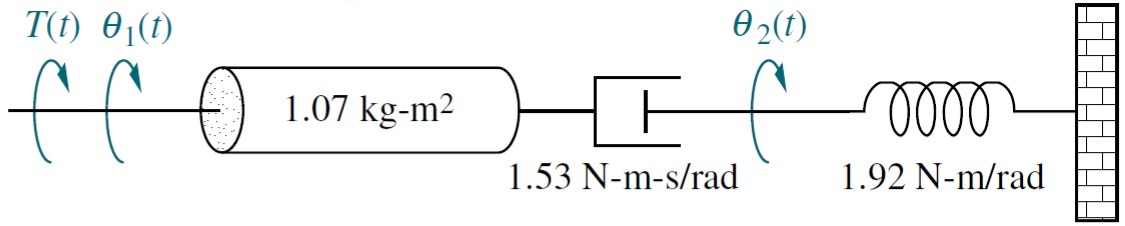
\includegraphics[ width = 0.8\textwidth]{fig_prob_02.jpg}
\end{figure}

\emph{Soluci\'on:} 
Tal como se indica en la sugerencia, si colocamos un cuerpo con inercia $I_\epsilon$ en el eje donde se mide $\theta_2(t)$ entonces las ecuaciones diferenciales son: 
\begin{align*}
1.07 \, \ddot{\theta}_1(t) \, 
& = \, T(t) + 1.53 \, ( \, \dot{\theta}_2(t) - \dot{\theta}_1(t) \, ) \\
I_{\epsilon} \, \ddot{\theta}_2(t) \, 
& = \, -1.53 \, ( \, \dot{\theta}_2(t) - \dot{\theta}_1(t) \, ) - 1.92 \, \theta_2(t)
\end{align*}
Ahora, tomando $I_{\epsilon} \approx 0$ y aplicando la transformaci\'on de Laplace de ambos lados de ambas equaciones tenemos: 
\begin{align*}
& ( \, 1.07 \, s^2 + 1.53 \, s \, ) \, \Theta_1(s) - 1.53 \, s \, \Theta_2(s) \, = \, T(s) \\
& 1.53 \, s \, \Theta_1(s) - ( \, 1.53 \, s + 1.92 \, ) \, \Theta_2(s) \, = \, 0
\end{align*}
Luego, de la segunda ecuaci\'on vemos que: 
\[
\Theta_1(s) \, = \, \left( \frac{ 1.53 \, s + 1.92 }{ 1.53 \, s } \right) \Theta_2(s)
\]
Consecuentemente, reemplazando la expresi\'on de arriba en la primera ecuaci\'on diferencial transformada, observamos que: 
\begin{align*}
& \left[ ( \, 1.07 \, s^2 + 1.53 \, s \, ) \left( \frac{ 1.53 \, s + 1.92 }{ 1.53 \, s } \right) 
- 1.53 \, s \right] \Theta_2(s) \, = \, T(s) \\[1ex]
& \Longrightarrow \; ( \, 1.07 \, s^2 + 1.34275 \, s + 1.92 \, ) \, \Theta_2(s) \, = \, T(s) \\[1ex]
& \Longrightarrow \; G(s) \; = \; 
\frac{1}{ 1.07 \, s^2 + 1.34275 \, s + 1.92 } \; \equiv \; \frac{ 0.9346 }{ s^2 + 1.25491 \, s + 1.7944 }
\end{align*}
Finalmente, reconociendo que $\omega_n = 1.34$ rad/s y $\zeta = 0.4684$, concluimos que las m\'etricas de respuesta en el tiempo de este sistema son: 
\begin{align*}
\% OS \, 
& = \, 100 \, \exp \left( -\frac{ \zeta \, \pi }{ \sqrt{1 - \zeta^2} } \right) 
\, = \, 18.9 \% \\[1ex]
T_p \, & = \, \frac{\pi}{ \omega_n \, \sqrt{1 - \zeta^2} } \, = \, 2.654 \: s \\[1ex]
T_s \, & = \, \frac{4}{ \zeta \, \omega_n } \, = \, 6.373 \: s
\end{align*}


\end{problem}
\vspace{\baselineskip}


\end{document}
